%-*-coding:utf-8;-*-
\documentclass[14pt]{beamer}
\usepackage[T1]{fontenc}
\usepackage[utf8]{inputenc}
%\usepackage[usenames,dvipsnames,svgnames,table]{xcolor}
\definecolor{links}{HTML}{2A1B81}
\hypersetup{colorlinks,linkcolor=,urlcolor=links}
\usetheme[numbering=none]{metropolis}           % Use metropolis theme
\setmainfont{Gentium}
\setsansfont{Gentium}
\hyphenation{me-mo-ra-bi-li-um}
\title{De corpore dramatum Latinorum in Croatia actorum restituendo}
\date{die 31 Julii 2018}
\author{Neven Jovanović}
\institute{Facultas philosophica Universitatis Zagrabiensis}
\begin{document}
  \maketitle
  


%% \begin{frame}
%% \tableofcontents
%% \end{frame}

\section{Prooemium: De dramatum in Croatia ignorantia et notitia}

\begin{frame}
  In Croatia ab anno 1525 usque ad annum 1805 plus quam sescentae actiones Latinae in scaena productae sunt.
\end{frame}

\begin{frame}
  Ubi id factum sit, et quorum ope?\\
  Qui libri impressi et manu scripti exsistunt?\\
  Qui dramatum tituli?\\
  Quid spectatores de actionibus iudicaverint?\\
\end{frame}

\begin{frame}
  Quare de dramatibus Latinis in Croatia tam diu nihil sciverimus, seu nihil scire voluerimus?
\end{frame}

\begin{frame}
Narratio: de Croatia, quae terra et ubi?
\end{frame}

\begin{frame}
Narratio: dramatum numerus et frequentia, productionum tempora et loca
\end{frame}

\begin{frame}
Narratio: ubi actiones ipsa sua absentia praefulgeant?
\end{frame}

\begin{frame}
Argumentatio: unde et quibus modis de dramatibus notitias hauriamus?
\end{frame}

\begin{frame}
Argumentatio: quomodo distinxerimus res de quibus fabulae agantur?
\end{frame}

\begin{frame}
  Argumentatio: exempla notitiarum typica et curiosa; exempla fabularum repetitarum
  
\end{frame}

\begin{frame}
  Peroratio: conclusiones quasdam, et quid porro faciendum et investigandum sit?
  
\end{frame}

\section{Prooemium: De ignorantiae quattuor causis}

\begin{frame}{Ignorantiae causae}
  \begin{itemize}
  \item textus dramatum deperditi
  \item dramata in scholis exhibita
  \item deest Auctor
  \item religio et ecclesia suspectae
  \end{itemize}
  
\end{frame}

\section{Narratio: De Croatia saeculis XVI-XIX}

{
    \usebackgroundtemplate{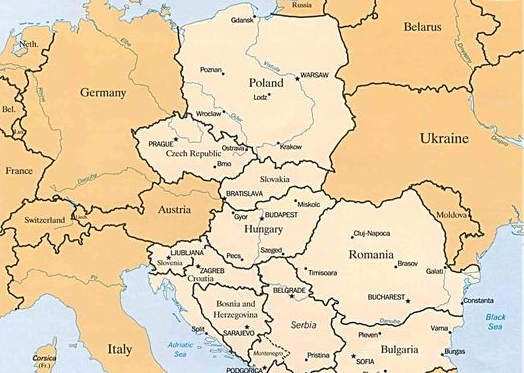
\includegraphics[width=\paperwidth]{img/centraleu2.jpg}}
    \setbeamertemplate{navigation symbols}{}
    \begin{frame}[plain]
    \end{frame}
    }

{
    \usebackgroundtemplate{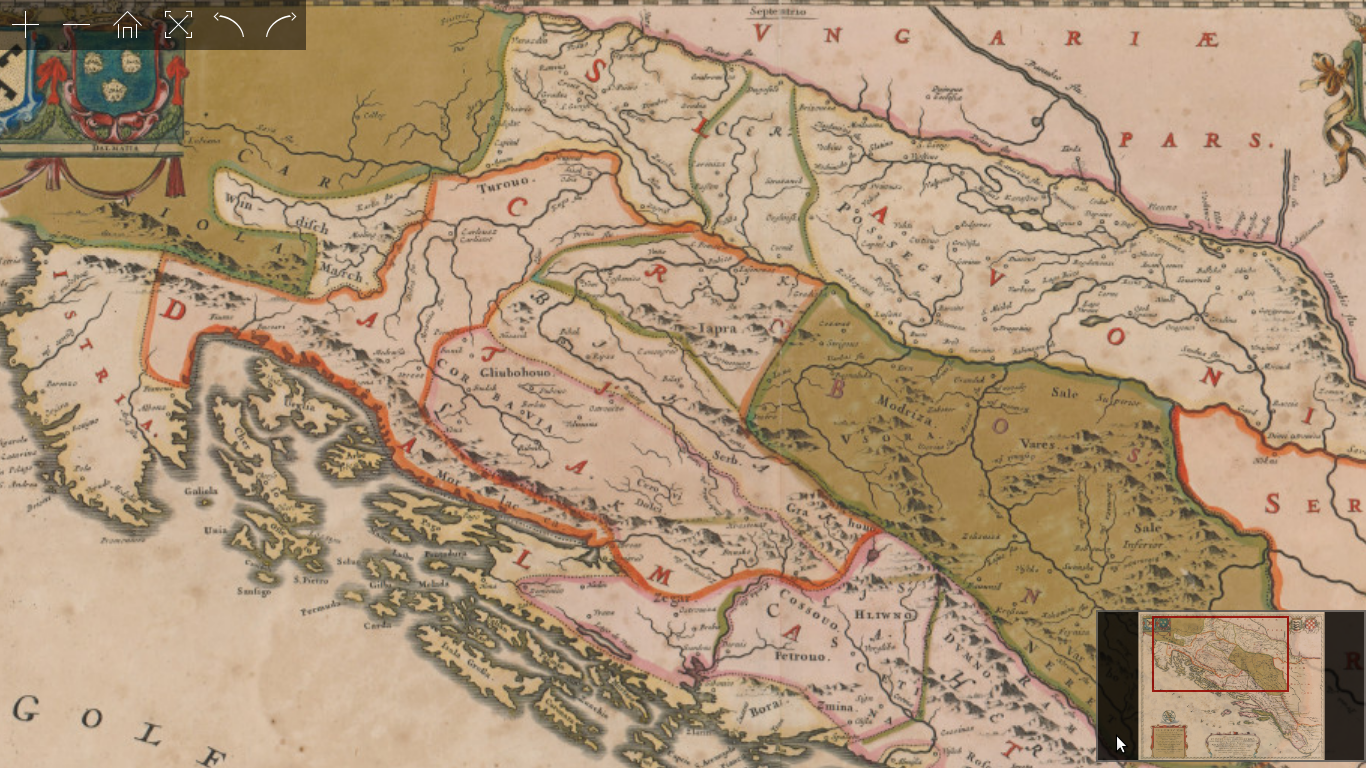
\includegraphics[width=\paperwidth]{img/illyricumhod.png}}
    \setbeamertemplate{navigation symbols}{}
    \begin{frame}[plain]
    \end{frame}
    }


\begin{frame}{Croatia inter dominationes divisa}

  \begin{itemize}
  \item Res publica Venetorum
  \item Provinciae hereditariae regni Austriaci
  \item   Ottomanicum imperium
  \item   Res publica Ragusina
  \item   Regnum Croatiae, Regnum Slavoniae
  \end{itemize}
\end{frame}


\begin{frame}{Societas Jesu in Croatia}
\begin{itemize}
  \item \alert{1559} venerunt Ragusam
  \item \alert{1604–1698} fundaverunt collegia Ragusae, Zagrabiae, Fluminis S. Viti (Rijeka), Varasdini, Posegae
  \item \alert{1773} suppressio ordinis
\end{itemize}
\end{frame}

{
    \usebackgroundtemplate{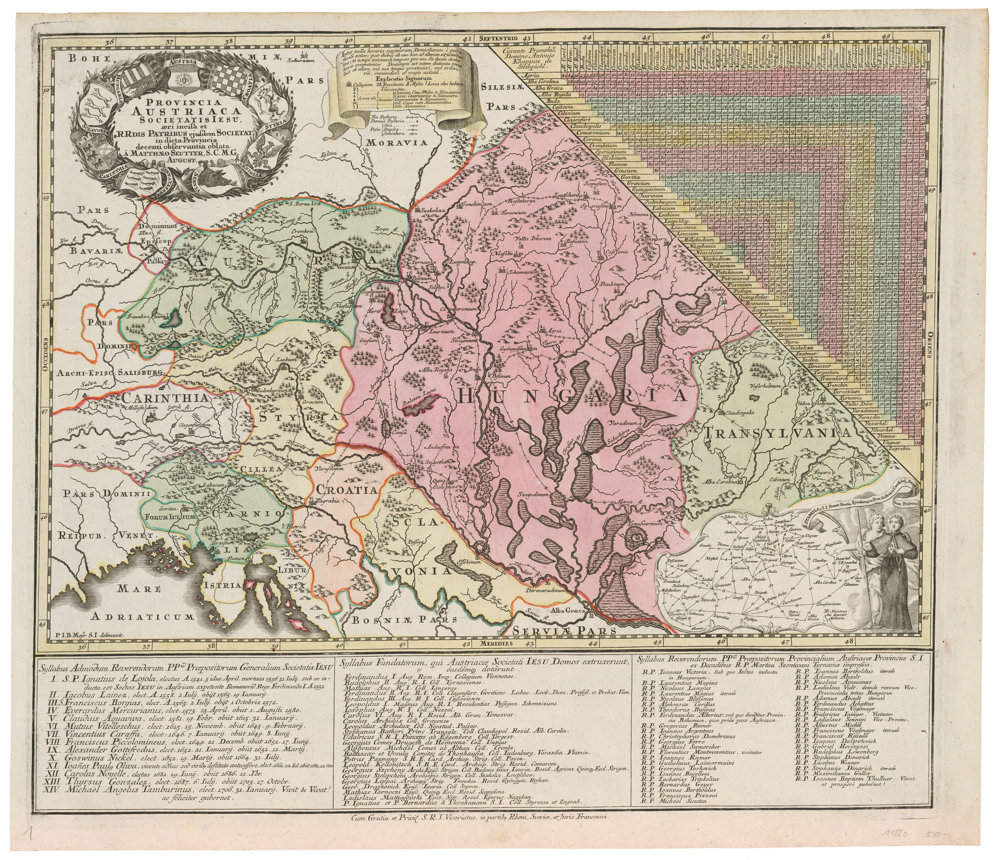
\includegraphics[width=\paperwidth]{img/eichler.jpeg}}
    \setbeamertemplate{navigation symbols}{}
    \begin{frame}[plain]
    \end{frame}
    }



\section{Narratio: quid, quando, ubi, quot?}


{
    \usebackgroundtemplate{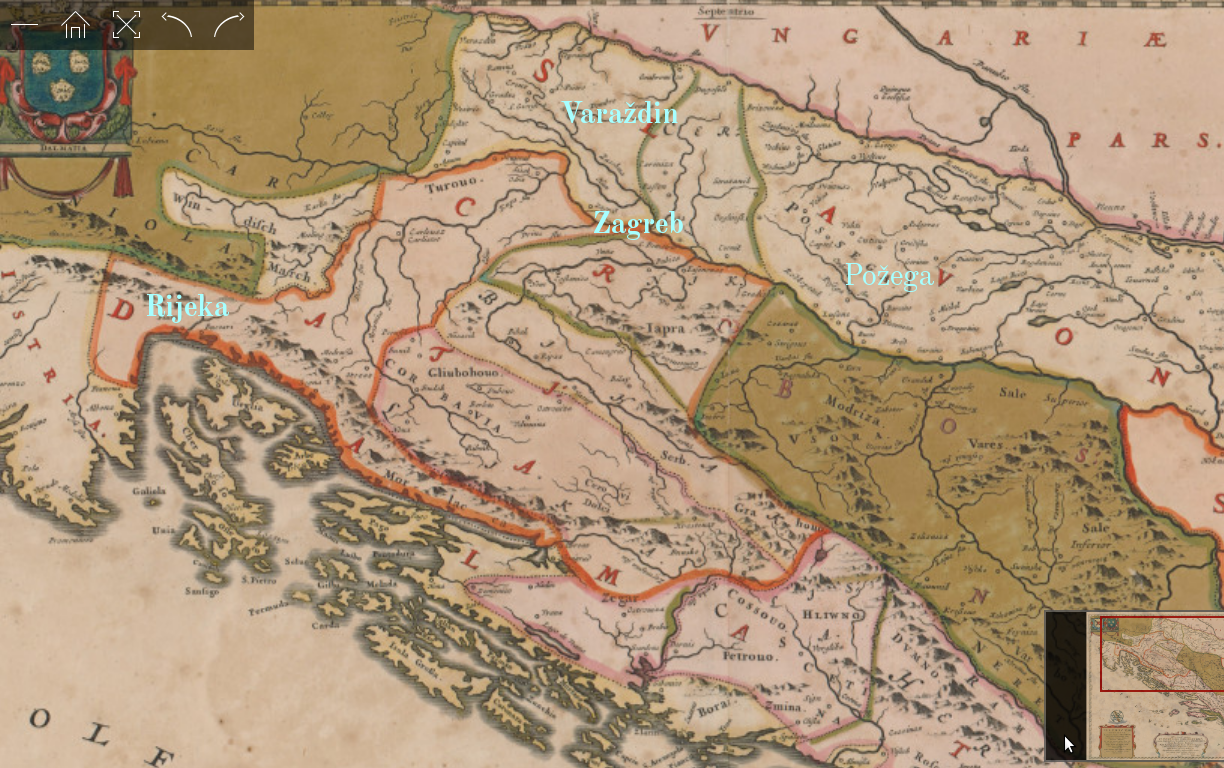
\includegraphics[width=\paperwidth]{img/illyricum_urb.png}}
    \setbeamertemplate{navigation symbols}{}
    \begin{frame}[plain]
    \end{frame}
}

{
    \usebackgroundtemplate{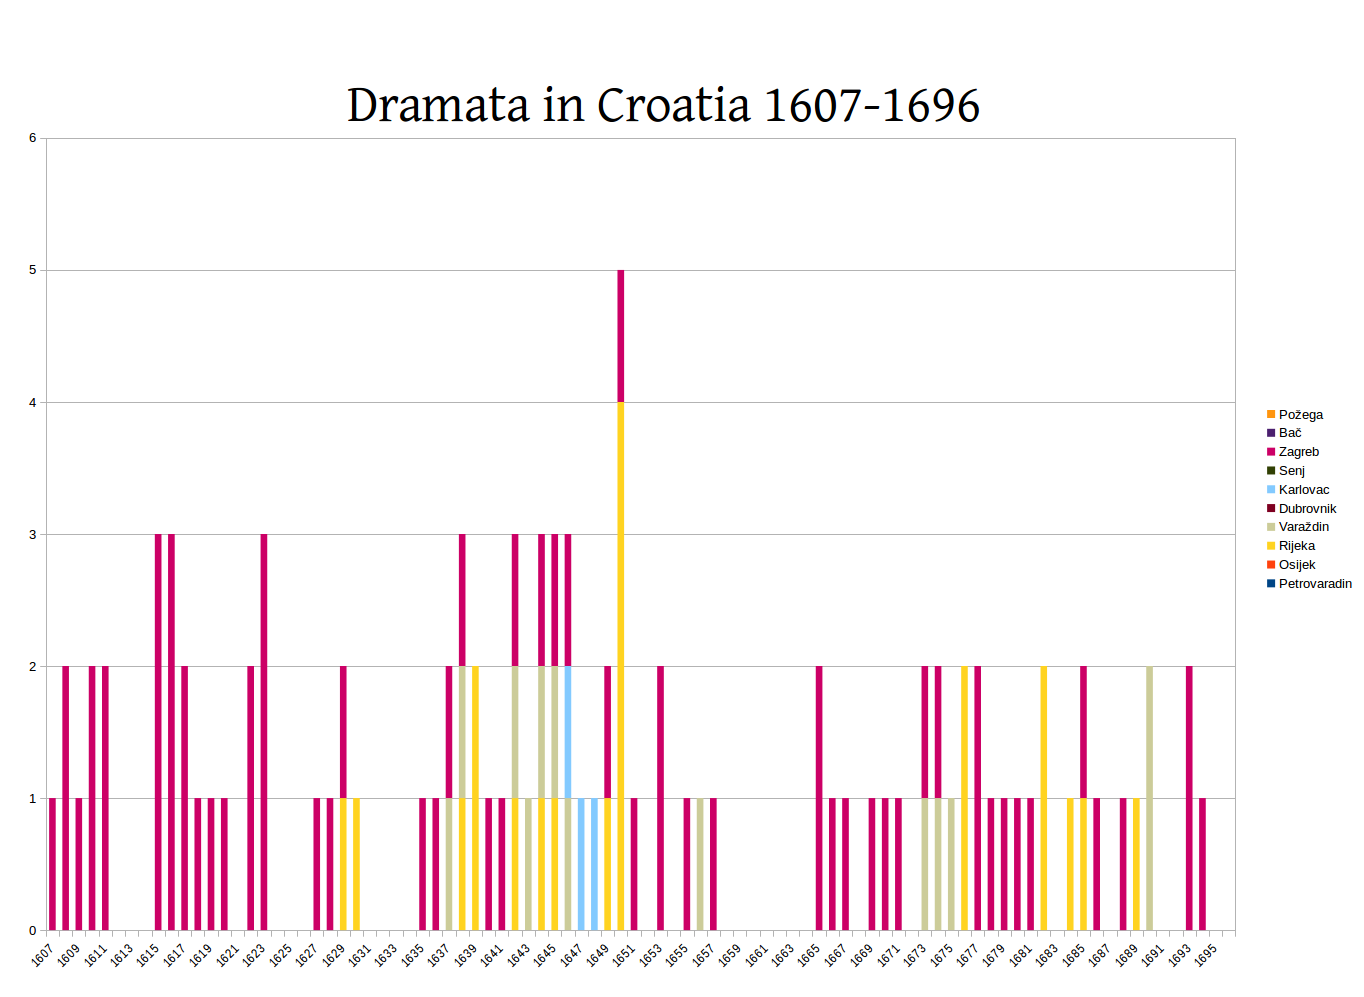
\includegraphics[width=\paperwidth]{img/drama17.png}}
    \setbeamertemplate{navigation symbols}{}
    \begin{frame}[plain]
    \end{frame}
}

{
    \usebackgroundtemplate{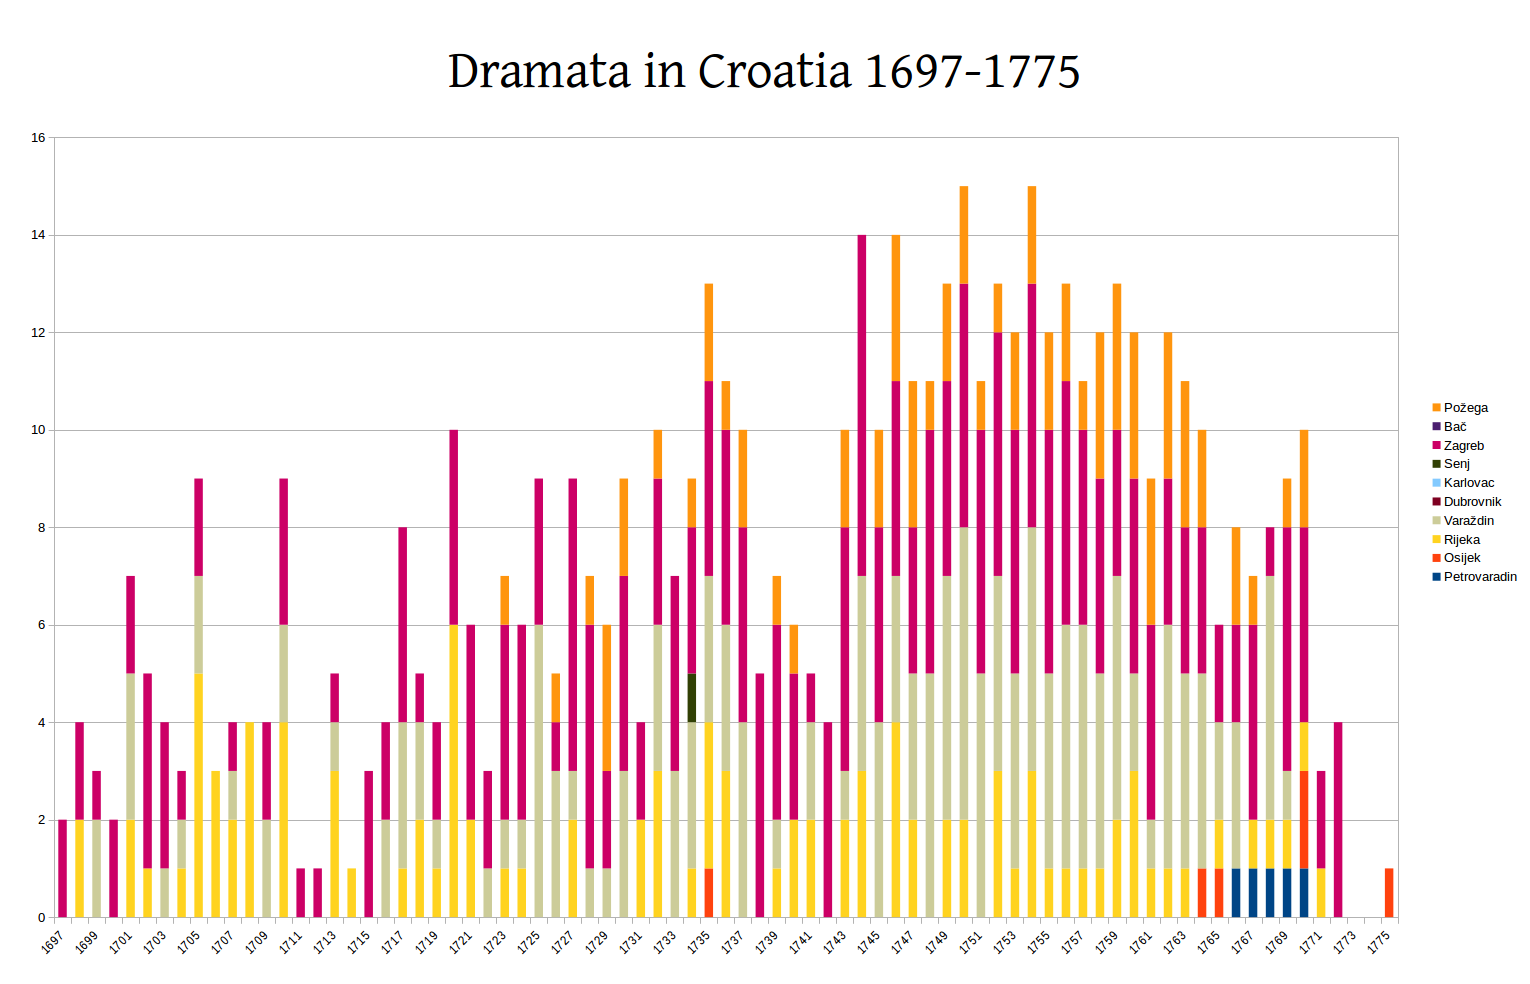
\includegraphics[width=\paperwidth]{img/drama18.png}}
    \setbeamertemplate{navigation symbols}{}
    \begin{frame}[plain]
    \end{frame}
}


\section{Argumentatio: unde et quomodo notitias hauserimus?}

\begin{frame}{Bibliographiae}

Martina Petranović and Lucija Ljubić. \emph{Repertoar hrvatskih kazališta : Knjiga peta : Deskriptivna obrada važnijih predstava na hrvatskom jeziku i izvedbi na stranim jezicima hrvatskih izvođača do 1840. godine}, Zagreb 2012.

Staud, Géza. \emph{A magyarországi jezsuita iskolai színjátékok forrásai, III. : 1561-1773, Fontes ludorum scenicorum in scholis S. J. Hungariae, pars tertia}, Budapest 1988.

\end{frame}
\begin{frame}{Historiae}

Fancev, Franjo, Građa za povijest školskog i književnog rada
isusovačkoga kolegija u Zagrebu. Starine. Knj. 37. Jugoslavenska
akademija znanosti i umjetnosti, Zagreb 1934.

Fancev, Franjo, Građa za povijest školskog i književnog rada
isusovačkoga kolegija u Zagrebu. Starine. Knj. 38. Jugoslavenska
akademija znanosti i umjetnosti, Zagreb 1937.

\end{frame}

\begin{frame}{Exemplum notitiae}

  \url{http://croala.ffzg.unizg.hr/basex/dramasingulare/croala.drama.d1e10078}
  
\end{frame}

{
    \usebackgroundtemplate{\includegraphics[width=\paperwidth]{img/alvarus.png}}
    \setbeamertemplate{navigation symbols}{}
    \begin{frame}[plain]
    \end{frame}
    }

\begin{frame}{Ex libris in computatrum}

Verba librorum > XML > receptaculum datorum > quaestiones XQuery

\end{frame}

{
    \usebackgroundtemplate{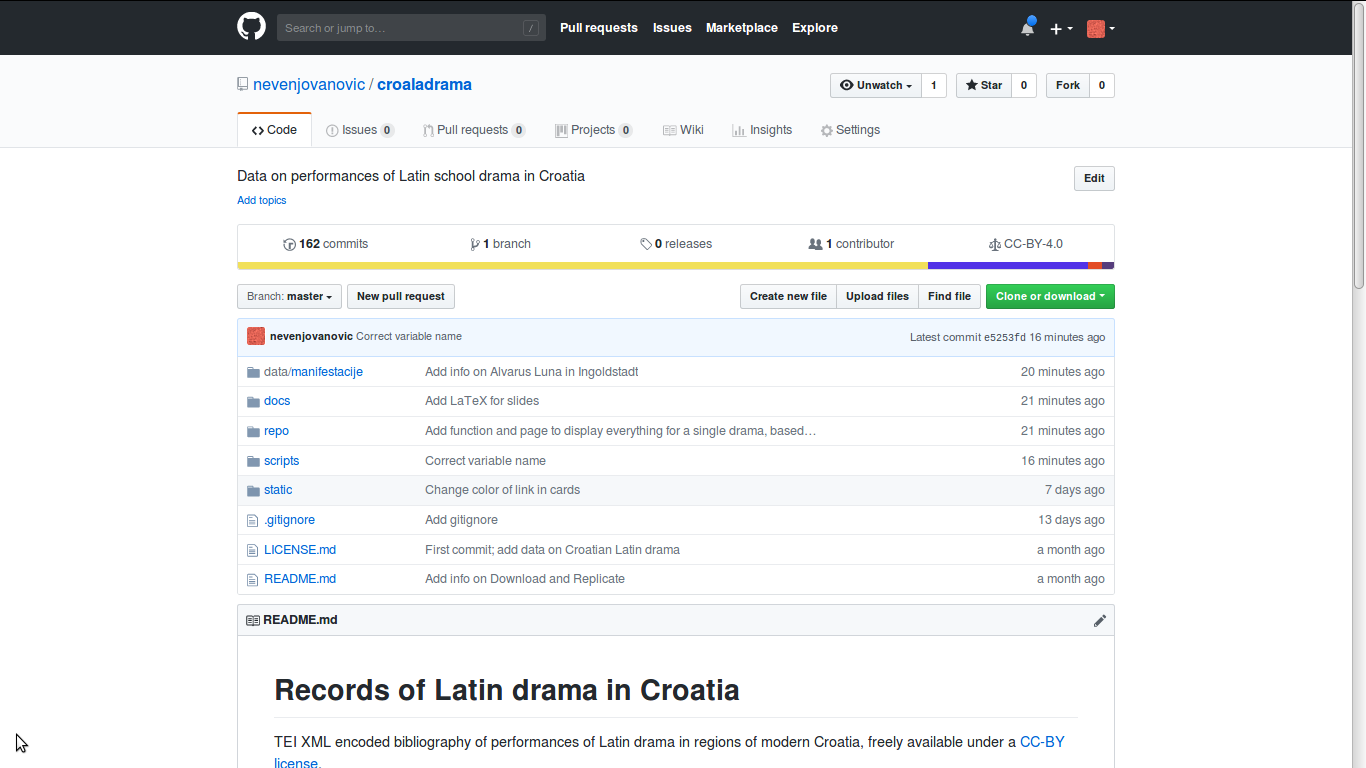
\includegraphics[width=\paperwidth]{img/drama_github.png}}
    \setbeamertemplate{navigation symbols}{}
    \begin{frame}[plain]
    \end{frame}
    }
\section{Argumentatio: exempla}

\begin{frame}{Gratulatio tumultuaria}
  \url{http://croala.ffzg.unizg.hr/basex/dramasingulare/croala.drama.d1e7315}
\end{frame}

\begin{frame}{Disputatio annalistarum}
  \url{http://croala.ffzg.unizg.hr/basex/dramasingulare/croala.drama.d1e14586}
\end{frame}

\begin{frame}{Erasmus Montanus drama Danicum}
  Datum Petrovardini 1769.

  Ad spectandum Erasmum Montanum Petrovardinum et vicinia tota adfuit et jure applausit.
  
  \url{http://croala.ffzg.unizg.hr/basex/dramasingulare/croala.drama.d1e49768}

  Ludovici Holberg drama Erasmus Montanus scriptum esse 1722, primum in scaena exhibitum 1747 dicitur.
    \end{frame}

\section{Argumentatio: dramata thematice}

\begin{frame}
  Heroes
\end{frame}

\begin{frame}{Qui heroes recurrunt saepissime?}
  Beata Virgo Maria\\
  Sanctus Ignatius\\
  David\\
  Sanctus Alexius\\
  Sanctus Ivanus Croatiae regis filius\\
  Sanctus Paulinus Nolanus\\
  Josephus Patriarcha\\
  Sanctus Stanislaus Kostka\\
  Carolus III Hispaniorum rex\\
  Selimus Turca
  
\end{frame}

\section{Peroratio: conclusiones}

\begin{frame}{De corpore dramatum Latinorum in Croatia}
  
\end{frame}

\begin{frame}{De corporibus et dramatibus comparandis}
  
\end{frame}

\begin{frame}{De corpore dramatum Europae proponendo}
  
\end{frame}

  \maketitle


\end{document}

